\documentclass[tikz,border=2mm]{standalone}
\usepackage[T1]{fontenc}
\usepackage{lmodern}
\usetikzlibrary{arrows.meta, shapes.geometric}

\begin{document}
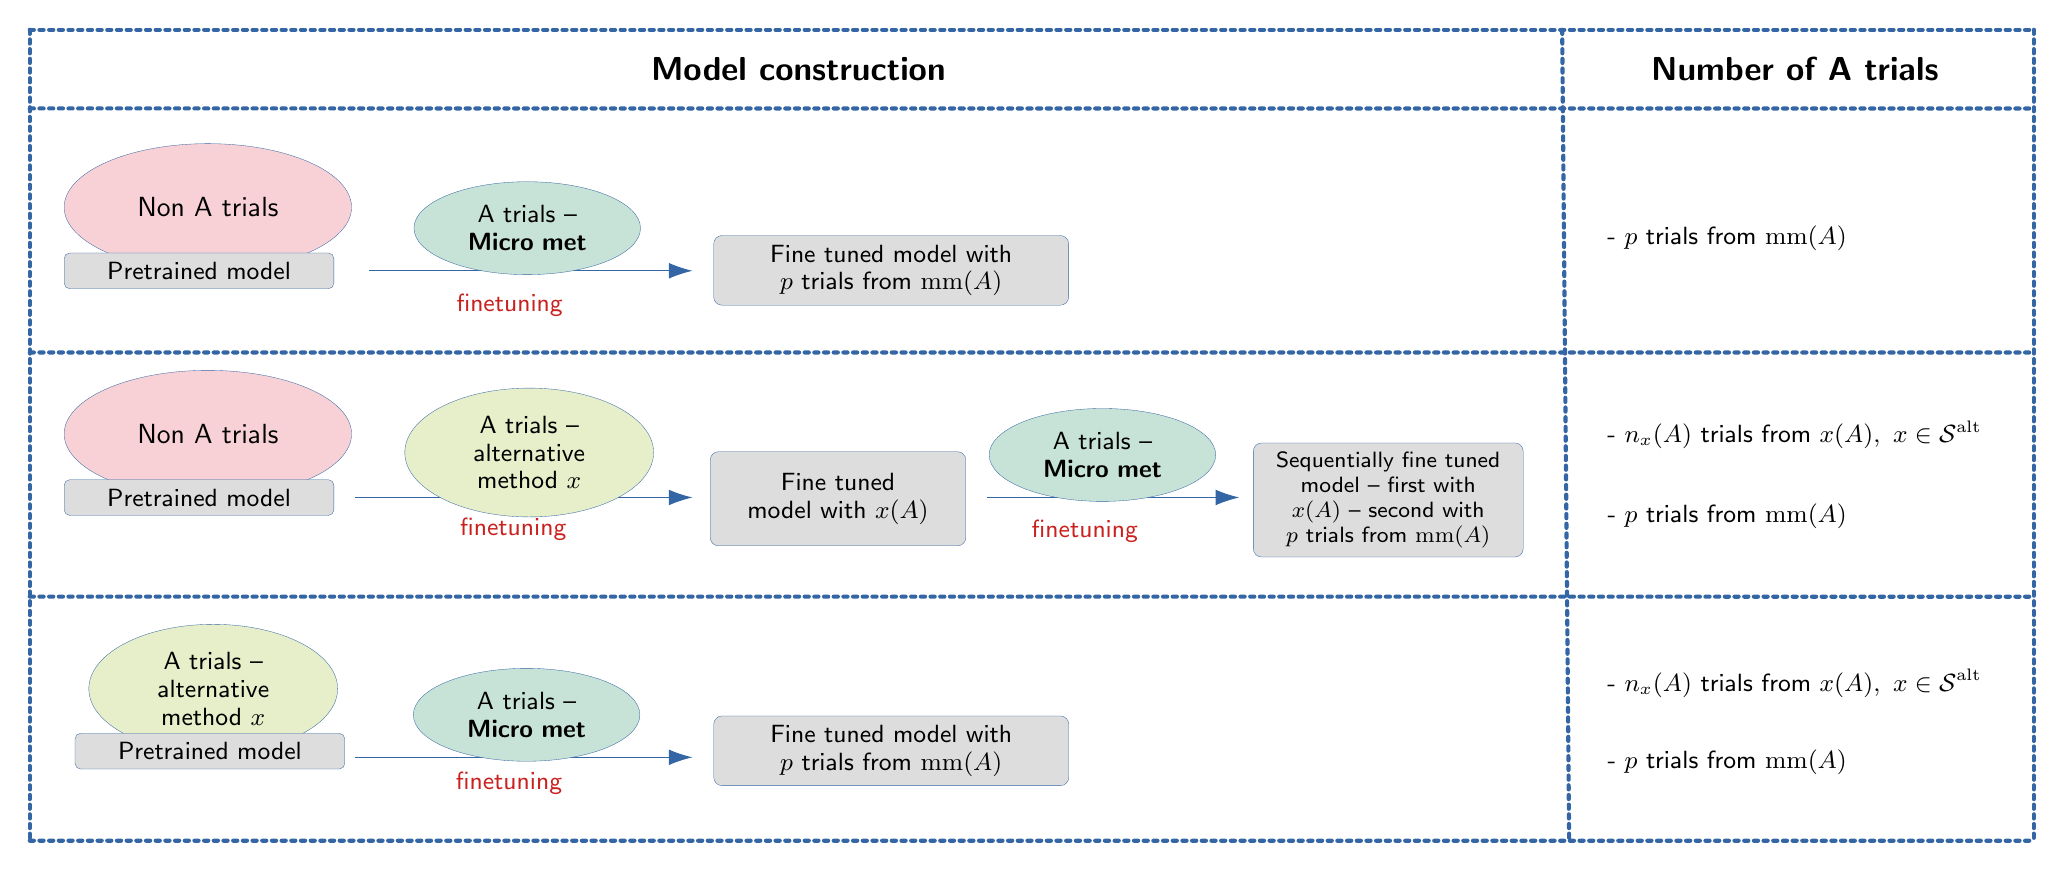
\begin{tikzpicture}[
  x=1cm,
  y=-1cm,
  font=\sffamily,
  >=Latex,
  blueLine/.style={draw=blueLine},
  nonA/.style={ellipse, blueLine, fill=nonAFill, line width=0.12pt,
               minimum width=3.65cm, minimum height=1.615cm,
               align=center, font=\sffamily\fontsize{10}{12}\selectfont},
  pretrained/.style={rounded corners=2pt, blueLine, fill=modelFill, line width=0.12pt,
                     minimum width=3.425cm, minimum height=0.323cm,
                     align=center, font=\sffamily\fontsize{9}{11}\selectfont},
  atrialsx/.style={ellipse, blueLine, fill=aXFill, line width=0.12pt,
                   minimum width=2.703cm, minimum height=1.25cm,
                   align=center, text width=2.0cm, font=\sffamily\fontsize{9}{10}\selectfont},
  atrialsmm/.style={ellipse, blueLine, fill=aMMFill, line width=0.12pt,
                    minimum width=2.48cm, minimum height=1.18cm,
                    align=center, text width=1.8cm, font=\sffamily\fontsize{9}{10}\selectfont},
  tuned/.style={rounded corners=3pt, blueLine, fill=modelFill, line width=0.12pt,
                minimum width=3.246cm, minimum height=1.195cm,
                align=center, text width=2.75cm, font=\sffamily\fontsize{9}{10}\selectfont},
  tunedmm/.style={rounded corners=3pt, blueLine, fill=modelFill, line width=0.12pt,
                  minimum width=4.508cm, minimum height=0.88cm,
                  align=center, text width=4.05cm, font=\sffamily\fontsize{9}{10}\selectfont},
  sequential/.style={rounded corners=3pt, blueLine, fill=modelFill, line width=0.12pt,
                     minimum width=3.427cm, minimum height=1.421cm,
                     align=center, text width=3.05cm, font=\sffamily\fontsize{8}{9}\selectfont},
  arrow/.style={blueLine, line width=0.35pt, -{Latex[length=3mm,width=2mm]}},
  sep/.style={blueLine, line width=1.5pt, dotted, line cap=round},
  finetune/.style={font=\sffamily\fontsize{9}{11}\selectfont, text=finetuneRed},
  note/.style={font=\sffamily\fontsize{9}{11}\selectfont, align=left},
  head/.style={font=\sffamily\fontsize{12}{14}\selectfont\bfseries, align=center}
]

\definecolor{blueLine}{RGB}{52,101,164}
\definecolor{nonAFill}{RGB}{247,209,213}
\definecolor{aXFill}{RGB}{231,238,202}
\definecolor{aMMFill}{RGB}{199,226,214}
\definecolor{modelFill}{RGB}{221,221,221}
\definecolor{finetuneRed}{RGB}{201,33,30}

% Coordinate system in centimeters from the upper-left corner, matching the ODG.

% Headers
\node[head, anchor=center] at (10.961,2.000) {Model construction};
\node[head, anchor=center] at (23.617,2.000) {Number of A trials};

% Separators
\draw[sep] (1.200,1.500) -- (26.650,1.500);
\draw[sep] (1.200,2.499) -- (26.650,2.500);
\draw[sep] (1.200,5.598) -- (26.650,5.599);
\draw[sep] (1.200,8.699) -- (26.650,8.700);
\draw[sep] (1.200,11.799) -- (26.650,11.800);
\draw[sep] (20.662,1.500) -- (20.750,11.800);
\draw[sep] (1.200,1.500) -- (1.200,11.800);
\draw[sep] (26.650,1.500) -- (26.650,11.800);

% Row 1: finetuning with mm(A)
\draw[arrow] (5.514,4.561) -- (9.617,4.561);
\node[nonA] at (3.462,3.754) {Non A trials};
\node[pretrained] at (3.350,4.562) {Pretrained model};
\node[atrialsmm] at (7.518,4.020) {A trials --\\\textbf{Micro met}};
\node[finetune, anchor=west] at (6.496,4.994) {finetuning};
\node[tunedmm] at (12.140,4.556) {Fine tuned model with $p$ trials from $\mathrm{mm}(A)$};
\node[note, anchor=west] at (21.113,4.148) {- $p$ trials from $\mathrm{mm}(A)$};

% Row 2: sequential finetuning with x(A), then mm(A)
\draw[arrow] (5.333,7.440) -- (9.616,7.440);
\draw[arrow] (13.359,7.440) -- (16.560,7.440);
\node[nonA] at (3.462,6.633) {Non A trials};
\node[pretrained] at (3.350,7.441) {Pretrained model};
\node[atrialsx] at (7.543,6.869) {A trials -- alternative method $x$};
\node[finetune, anchor=west] at (6.542,7.839) {finetuning};
\node[tuned] at (11.465,7.456) {Fine tuned\\model with $x(A)$};
\node[atrialsmm] at (14.823,6.900) {A trials --\\\textbf{Micro met}};
\node[finetune, anchor=west] at (13.801,7.873) {finetuning};
\node[sequential] at (18.453,7.472) {Sequentially fine tuned model -- first with $x(A)$ -- second with $p$ trials from $\mathrm{mm}(A)$};
\node[note, anchor=west] at (21.113,6.646) {- $n_x(A)$ trials from $x(A),\ x\in\mathcal{S}^{\mathrm{alt}}$};
\node[note, anchor=west] at (21.114,7.673) {- $p$ trials from $\mathrm{mm}(A)$};

% Row 3: finetuning with mm(A) from an x(A)-based pretrained model
\draw[arrow] (5.333,10.740) -- (9.616,10.740);
\node[atrialsx] at (3.530,9.869) {A trials -- alternative method $x$};
\node[pretrained] at (3.488,10.662) {Pretrained model};
\node[atrialsmm] at (7.510,10.200) {A trials --\\\textbf{Micro met}};
\node[finetune, anchor=west] at (6.488,11.073) {finetuning};
\node[tunedmm] at (12.141,10.657) {Fine tuned model with $p$ trials from $\mathrm{mm}(A)$};
\node[note, anchor=west] at (21.113,9.8) {- $n_x(A)$ trials from $x(A),\ x\in\mathcal{S}^{\mathrm{alt}}$};
\node[note, anchor=west] at (21.114,10.8) {- $p$ trials from $\mathrm{mm}(A)$};

\end{tikzpicture}
\end{document}
